% !TEX TS-program = pdflatex
% !TEX encoding = UTF-8 Unicode

\documentclass[12pt]{refart} % use larger type; default would be 10pt
\usepackage{imakeidx}
\usepackage{comment}
%\usepackage[utf8]{inputenc} % Required for inputting international characters
%\usepackage[T1]{fontenc} % Output font encoding for international characters

%\usepackage{mathpazo} % Palatino font

%%% PAGE DIMENSIONS
%\usepackage{geometry} % to change the page dimensions
%\geometry{a4paper} % or letterpaper (US) or a5paper or....
%\geometry{margin=1in} % for example, change the margins to 2 inches all round
% \geometry{landscape} % set up the page for landscape
%   read geometry.pdf for detailed page layout information

\usepackage{graphicx} % support the \includegraphics command and options

% \usepackage[parfill]{parskip} % Activate to begin paragraphs with an empty line rather than an indent

%%% PACKAGES
\usepackage{booktabs} % for much better looking tables
\usepackage{array} % for better arrays (eg matrices) in maths
\usepackage{paralist} % very flexible & customisable lists (eg. enumerate/itemize, etc.)
\usepackage{verbatim} % adds environment for commenting out blocks of text & for better verbatim
\usepackage{subfig} % make it possible to include more than one captioned figure/table in a single float
\usepackage{amsmath}
\usepackage{float}

\usepackage{gensymb}
% These packages are all incorporated in the memoir class to one degree or another...

\usepackage{listings} % for including code 
\usepackage{color}
\usepackage[dvipsnames]{xcolor}

\lstdefinestyle{VHDLMeUp}{
	basicstyle=\scriptsize,
	caption=\lstname, 
	keywordstyle=\color{blue},
	stringstyle=\color{red},
	commentstyle=\color{gray}
    language=VHDL
}

\newenvironment{fullfigure}
{\begin{figure} [H]
\hspace*{-\leftmarginwidth}%
\begin{minipage}{\fullwidth}}
{\end{minipage}\end{figure}}
	
%%% HEADERS & FOOTERS
%\usepackage{fancyhdr} % This should be set AFTER setting up the page geometry
%\pagestyle{fancy} % options: empty , plain , fancy
%\renewcommand{\headrulewidth}{0pt} % customise the layout...
%\lhead{Sophia Liu}\chead{}\rhead{EE52 documentation}
%\lfoot{}\cfoot{\thepage}\rfoot{}

\usepackage{hyperref} % for links

\pagestyle{myfootings}

\title{Digital Oscilloscope Documentation}
\author{Sophia Liu \\
	EE 52 \\
	Spring 2017}
\date{} % Activate to display a given date or no date (if empty),
         % otherwise the current date is printed 
\makeindex

\begin{document}
%\maketitle 
\begin{fullpage}
\begin{titlepage} % Suppresses displaying the page number on the title page and the subsequent page counts as page 1
	\newcommand{\HRule}{\rule{\linewidth}{0.5mm}} % Defines a new command for horizontal lines, change thickness here
	
	\center % Centre everything on the page
	
	%------------------------------------------------
	%	Headings
	%------------------------------------------------
	
	%\textsc{\LARGE Institution Name}\\[1.5cm] % Main heading such as the name of your university/college
	
	\textsc{\Large EE 52}\\[0.5cm] % Major heading such as course name
	
	\textsc{\large Spring 2017}\\[0.5cm] % Minor heading such as course title
	
	%------------------------------------------------
	%	Title
	%------------------------------------------------
	
	\HRule\\[0.4cm]
	
	{\huge\bfseries Digital Oscilloscope Documentation}\\[0.4cm] % Title of your document
	
	\HRule\\[1.0cm]
	
	%------------------------------------------------
	%	Author(s)

	{\large
	\textsc{Sophia Liu}} % Your name
	
	%------------------------------------------------
	%	Date
	%------------------------------------------------
	
	\vfill\vfill\vfill % Position the date 3/4 down the remaining page
	
	{\large\today} % Date, change the \today to a set date if you want to be precise
	
	%------------------------------------------------
	%	Logo
	%------------------------------------------------
	
	%\vfill\vfill
	%\includegraphics[width=0.2\textwidth]{placeholder.jpg}\\[1cm] % Include a department/university logo - this will require the graphicx package
	
	%----------------------------------------------------------------------------------------
	
	\vfill % Push the date up 1/4 of the remaining page
	
\end{titlepage} 
\end{fullpage}

\tableofcontents

\newpage 
\section{User Manual} % ADD PICS! 
\begin{comment}
	How to use system (how it works or as if it worked) 
Non-technical, written for user
"screen" shots are useful - display output pics 
Keypad layout (switch) - also on pcb 
Usually ~10 pages 
\end{comment}
\subsection{System Description}
The System on Programmable Chip (SoPC) Digital Oscilloscope is an FPGA/microprocessor-based system capable of capturing and displaying up to 5 MHz signals. The analog input can range from 0 V to 3.8 V. The system has all the features of a standard oscilloscope with the exception of input signal scaling. Two rotary encoders are used to control the settings, and a LCD display is used to display the captured signal.  

\subsection{How to Use the System} 
The system will begin immediately upon powering up. \footnote{The serial configuration device currently does not work, so the FPGA must first be programmed through the JTAG debugger.} The system starts in one-shot trace mode with a sampling rate of 100 ns, a mid-level trigger (halfway between the minimum and maximum trigger levels, at  1.9 V) with no delay and positive slope, and with the menu displayed and scale set to axes. % STARTUP PIC
The probe can be attached to the desired input source. The oscilloscope settings are described in section~\ref{subsec:SystemSettings}. The reset button can be used to restart the system. 
%ROTARY ENCODERS LABELED, RESET BUTTON

\subsection{System Settings}\label{subsec:SystemSettings}

% ADD MENU PICS
\subsubsection{Menu}\index{Menu}
The scope parameter menu is located in the upper right corner of the LCD and contains the following entries in order:

\begin{verbatim}
Mode
Scale
Sweep
Trigger
    Level
    Slope
    Delay
\end{verbatim}

The menu display can be toggled on and off by pressing the menu rotary encoder. The user can cursor to any of the entries by turning the menu rotary encoder and can change a setting by turning the secondary rotary encoder. Changes take effect immediately. More rotary details can be found in section~\ref{subsubsec:RotaryEncoderFunctionality}. The menu entries are described in more detail below.

\begin{description}
	\index{Menu!Mode}\item[Mode]The Mode menu entry can be set to Mode Normal, Mode Automatic, or Mode One-Shot. In Mode Normal the scope waits for another trigger after every retrace. In this mode, new traces are captured as fast as the scope can redraw the screen. Mode Automatic works the same as Mode Normal if there are trigger events. But if no trigger event occurs after a specified delay (typically significantly longer than the time represented by a screen of data) the scope triggers automatically without a trigger event occurring. In Mode One-Shot the scope triggers only once and then holds that trace on the screen. It does not look for another trigger event until the Trigger menu item is selected and secondary rotary encoder is turned.
	
	\index{Menu!Scale}\item[Scale] The Scale menu entry can be set to Scale Axes, Scale Grid, or Scale Off. If the scale is set to Scale Axes, the x and y axes are displayed along with the trace. If the scale is set to Scale Grid, an x-y grid is displayed along with the trace. If the scale is set to Scale Off, no axes or grid are displayed.
	
	\index{Menu!Sweep}\item[Sweep] The Sweep menu entry sets the sweep rate (in time per sample) for the scope. Possible settings are: 100, 200, and 500 nanoseconds, and 1, 2, 5, 10, 20, 50, 100, 200, and 500 microseconds, and 1, 2, 5, 10, and 20 milliseconds (per sample).
	
	\index{Menu!Trigger}\item[Trigger] The Trigger menu entry re-arms the trigger for the scope in one-shot mode. Any time it is selected and the secondary rotary encoder is turned the scope trigger is re-armed and a new trace will then be captured once the trigger conditions (level and slope) are met.
	
	\index{Menu!Level}\item[Level] The Level menu entry sets the trigger level. It can be set to any value from the most negative input voltage to the most positive in 128 steps. Additionally, the trigger level is displayed as a line on the screen when the trigger level is being changed.
	
	\index{Menu!Slope}\item[Slope] The Slope menu entry is either Slope + or Slope - and determines whether the scope is triggered on a positive or negative slope respectively.
	
	\index{Menu!Delay}\item[Delay] The Delay menu entry determines the trigger delay. It sets the time after the trigger event at which the trace will start. It may be set to any value from the minimum delay to the maximum delay times the sample rate and it is displayed as a time.
\end{description}

\subsubsection{Rotary Encoder Functionality} \index{Rotary Encoder Functionality} \label{subsubsec:RotaryEncoderFunctionality}
The user can change the scope configuration via two rotary encoders (seen in \ref{}). All of the scope parameters are set via an on-screen menu. The rotary actions are detailed below: 
% ADD BOARD LAYOUT WITH ROTARY ENCODERS LABELED
\begin{description}
	\item[Press encoder 1] Turns the menu on/off. If the menu is off it is not displayed and turning the rotary encoders have no effect on the settings.
	
	\item[Turn encoder 1 CW] Moves the cursor down, if not already at the bottom menu item. If at the bottom, the cursor does not move. 
	
	\item[Turn encoder 1 CCW] Moves the cursor up, if not already at the top menu item. If at the top, the cursor does not move.
	
	\item[Turn encoder 2 CW] Changes the currently selected (with cursor) menu item. Goes "forward" through the list of possible settings. If at the "end" of the list, doesn't change the current selection.
	
	\item[Turn encoder 2 CCW] Changes the currently selected (with cursor) menu item. Goes "backward" through the list of possible settings. If at the "beginning" of the list, doesn't change the current selection.
\end{description}

%IS THERE ANYTHING ELSE? IDK 

\section{Technical Documentation} 
\subsection{Hardware} 
\subsubsection{Hardware System Overview} 
\begin{comment}
			System overview 
	Very high level description
	Use block diagram 
	Describe how the system works and how blocks interact 
	Easiest to describe in terms of UI interactions 
	Can be multi-level (may not need that much detail at system level) 
	Ex: how signal moves through scope to get to display 
	1-2 pages of text
\end{comment}
% BLOCK DIAGRAM
% BOARD LAYOUT
% MEMORY MAP
The oscilloscope system is centered around a Cyclone III FPGA, which includes a Nios II CPU and controllers for the VRAM, LCD, rotary encoders, and analog input and triggering. Upon startup, the bitmap %TODO is it a bitmap???
is loaded from the serial EEPROM. The %SOFTWARE? 
is then loaded from the ROM.

\marginlabel{Receiving a Signal:} When the probe is connected to a desired input, the analog signal is sent to an Analog to Digital Converter chip. 8 bits of data are then sent in parallel to the FPGA to an analog controller. The various trigger setting inputs (auto triggering, trigger enable, trigger slope, trigger level) are used along with the 8 bit signal to determine if the system should begin sampling. Once triggering has occurred, the signal is written to a %SIZE, 512 
FIFO buffer at the sampling rate. Once the FIFO is full, the CPU clocks out and stores the buffer data to be displayed. 

\marginlabel{Displaying a Signal:} In order to display the signal on the LCD, data is written to the VRAM, which is then sent out to the LCD. Several control signals (write enable, chip select, address, wait) are sent from the CPU to the VRAM controller to perform read and write operations on the VRAM. A (moore??) state machine is used to generate 

\subsubsection{Power} \index{Power} \label{subsec:Power}
%TODO REFERENCE SCHEMATIC 
A din4 connector (PWR1) is used to supply the board with +/-12 V and 5 V. All chips are locally bypassed (...?)

5 V is used to power the reset, VRAM, SRAM, ROM, and ADC chips. 

Several LM1086 regulators are used to generate the other required voltages. Specifically, U14 uses the 5 V supply to generate 2.5 V for analog power to the FPGA PLLs, and U15 uses the 5 V supply to generate 1.2 V for FPGA power supply and digital power to the FPGA PLLs. U16 generates 3.3 V from 5 V, which is used to power the FPGA I/O supply pins, buffers, JTAG, serial configuration device, clock, and for pulling high the rotary encoders. (??) 

Regulators also generate 5 V from 12 V (U24) and 4 V from 5 V (U23) for ADC reference voltages. (more analog stuff in analog section?) 

A boost converter is used to generate the 25 V necessary for the LED backlight. U21 (part number AP3012) steps up from 5 V and outputs 25 V. (more detail? was used because?)

\subsubsection{Analog System}\index{Analog!Hardware} \label{subsec:AnalogHardware}
The analog input can range from 0 to 4 V. An analog-to-digital converter (U17, TLC5510A) was used to digitize the input signal to 8 bits. This was chosen because of the simplicity of the circuit needed in order to meet the 0-3 V requirement.

Several analog supply voltages were used to isolate the analog and digital circuitry. An external 4 V analog reference was generated and used for a 0-4 V range for the input signal. A 5 V analog supply voltage was also required, along with an analog ground reference connected to digital ground through an inductor. %TODO schematic 

\marginlabel{Analog logic:}
\index{Analog!Logic}

\marginlabel{Analog inputs:}
Several values are taken as outputs from the software and are used in the hardware logic. Specifically, an 8 bit trigger level, 1 bit auto triggering, 1 bit trigger slope, 1 bit trigger enable, 19 bit sampling rate, and 16 bit trigger delay are used.  
%TODO blocks quartus pic

%TODO quartus pics
\marginlabel{Trigger logic:} \index{Trigger}
First, the system determines whether or not a trigger has occurred.
A Moore state machine is used to determine whether or not a trigger has occurred. It sets the the trigger event signal high when the trigger slope is positive and the signal has transitioned from below to above the trigger level, or if the trigger slope is negative and the signal has transitioned from above to below the trigger level. The code can be found in Appendix~\ref{scopetrig.vhd}.%TODO different way of quoting code??

Thus, the 8-bit signal is compared to the trigger level, and the less than and equal to outputs are sent to the trigger state machine along with the trigger slope. 

\index{Trigger!Autotrigger} 
The system also generates a trigger event if auto trigger is enabled after 512 clocks, which was arbitrarily chosen as a short amount of time. %TODO chosen because? maybe better to set auto trigger to # samples

A counter and comparator are used to create a clock at the given sampling rate. Once a trigger event has occurred, another counter and comparator are used to create the trigger delay. The signal is then written into a FIFO buffer at the sampling rate, which is clocked out through the software when it is full. The FIFO has a size of 480 words, or the length of the LCD. 

%TODO describe reasons

\subsubsection{Rotary Encoders}\index{Rotary Encoders} \label{subsec:Rotary}%TODO reorder? 
Two rotary encoders are used for the user input. %TODO pics 
These include and A and B output for the encoder and a single pull single throw push button switch. 

Pins A and B are pulled high\footnote{1 K resistors were used in place of the 10 K resistors on the schematic because the voltage high output was too low for the buffers.}, while the common pin is grounded to create out-of-phase pulses from outputs A and B. 
%TODO wave diagram
%TODO schematic pics 


\marginlabel{Rotary decoder logic:} 
The rotary logic block consists of a debouncer for the push button and a decoder for the rotary encoder. %TODO debouncer, decoder pics 

The debouncer (AnalogDebounce) takes as inputs the active-low button input (Rotary1\_P and Rotary2\_P on the schematic), clock, and active-low reset signal. It outputs a single active-high clock pulse whenever the button input signal is low for longer than 100000 clocks, which was chosen through testing the switches. 

The decoder (RotaryController) takes as inputs the two active-low outputs from the encoder (Rotary1\_A and Rotary1\_B, and Rotary2\_A and Rotary2\_B on the schematic), and the reset and clock signals, and outputs a single active-high clock pulse for each counter-clockwise turn of the rotary encoder, where output A leads B. %TODO a leading b/one ccw turn figure

This is accomplished by first debouncing the input using a counter and comparator to eliminate glitches. Several DFFs are used in series in order to read inputs A and B from two consecutive clocks to determine when edges have occurred. An SRFF is set low when input B goes from low to high while input A is still low, and is set high otherwise. The inverse of this is returned as the output, resulting in a decoder for one direction. Two decoders are used for each rotary encoder to distinguish clockwise and counterclockwise turns. 
%TODO more pics, of rotary block

\subsubsection{VRAM and LCD}\index{VRAM}\index{LCD} \label{subsec:VRAMLCD}
Two 256Kx4 DRAM with 512x4 SAM (serial access memory) chips (U19, U22, MT42C4225) were used for a total of 8 bits of data, with a 480x272 RGB TFT LCD (Connector J2, ER-TFT043-3).
%TODO schematic  pic

%TODO vram lines


\marginlabel{VRAM:} \index{VRAM}
Each VRAM sends 4 bits of serial data to the LCD, and receives 4 bits of data from the CPU, along with a 9 bit address and row address strobe (RAS), column address strobe (CAS), write enable (WE),and output enable (OE) signals from the VRAM controller. A serial clock signal is also sent to the VRAM. The LCD controller generates the various clock signals that are sent to synchronize the VRAM and LCD. 

The VRAM consists of the DRAM, transfer circuitry, and SAM. Read and write cycles are performed to read and write to the DRAM, and read transfer cycles are performed to transfer a row from the DRAM to SAM. 
 %TODO serial write
The VRAM is refreshed when no other operations are being performed to retain data. 

The two chips are sent the same control and address signals, and receive and output different data signals. 

memory,sam stuff

\marginlabel{LCD:} \index{LCD}
The LCD receives 8 bits of data in parallel from the DRAM, 3 bits of red, 3 bits of green, and 2 bits of blue, with the unused color bits pulled down. It also receives a horizontal sync, vertical sync, clock, and data enable signal from the LCD controller. The touch inputs were unused. 
%TODO block diagram 

The LCD also required a 25V backlight supply (VLED on the schematic). A step-up converter (U21) was used, which is discussed in more detail in Section~\ref{subsec:Power}.  

\marginlabel{Logic overview:}
The VRAM-LCD system consists of a VRAM controller and LCD controller that interact with each other, the CPU, and the VRAM and LCD.

\begin{fullfigure} 
	\centering
	\includegraphics[width=1\textwidth]{{data/VRAM_LCD_Block.png}}
	\caption{Block Diagram for VRAM and LCD.}
	\label{Block:VRAM_LCD}    
\end{fullfigure}

\begin{fullfigure} 
	\centering
	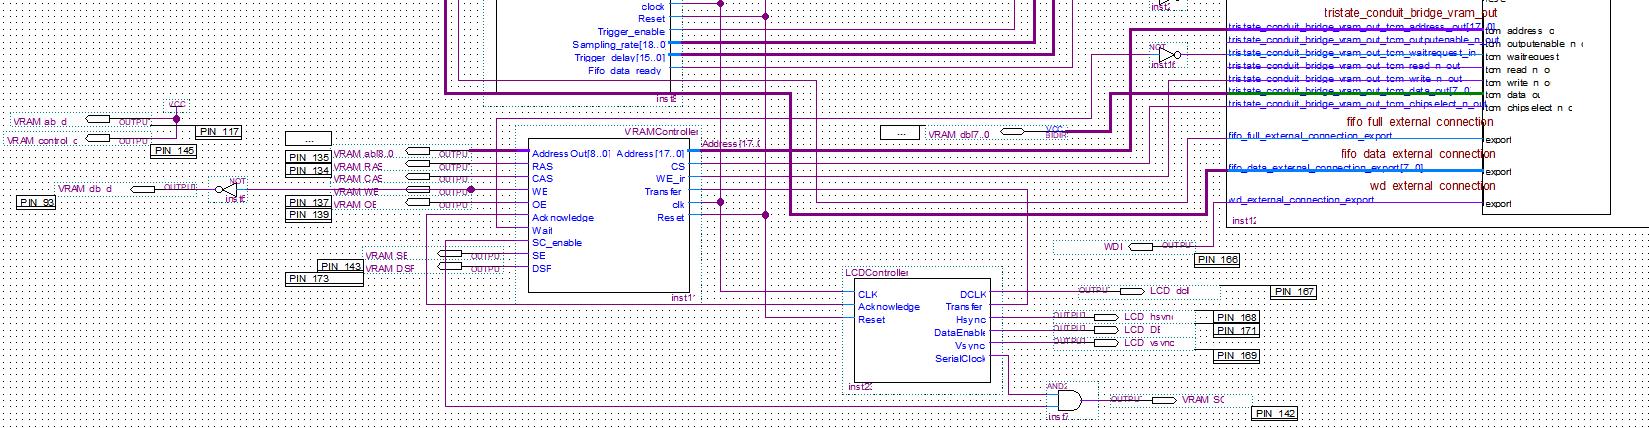
\includegraphics[width=1\textwidth]{{data/VRAMCPU.png}}
	\caption{VRAM and LCD Controllers.}
	\label{Block:VRAM_CPU}    
\end{fullfigure}

\marginlabel{VRAM Controller:} \index{VRAM! Controller}
The VRAM controller takes several inputs from the CPU: 1-bit chip select and write enable signals, and an 18-bit address. It also takes as an input a transfer request signal from the display controller. A state machine is used to generate the output signals, the RAS, CAS, address selector, WE, OE, serial clock, CPU wait output, and transfer acknowledge signals.

\begin{fullfigure} 
	\centering
	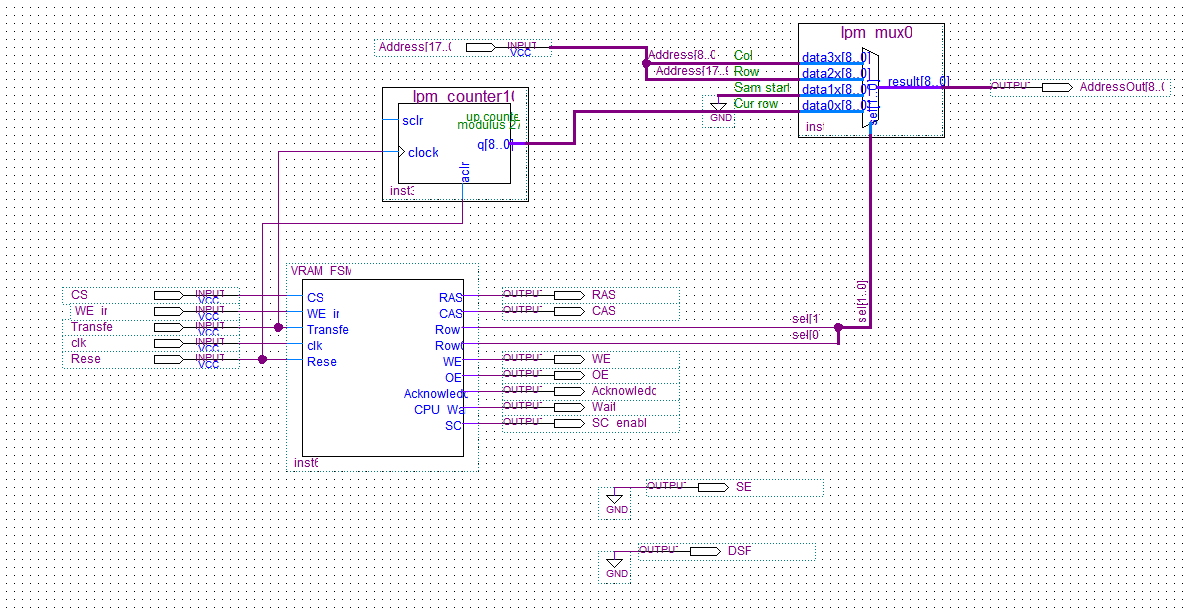
\includegraphics[width=1\textwidth]{{data/VRAM_Controller.png}}
	\caption{VRAM Controller.}
	\label{Block:VRAM_Controller}    
\end{fullfigure}


%mux address 
The output address is selected and outputted using a multiplexer. For %TODO cycles 
either the column or row, the first or second half of the input address, is returned. In the case of a row transfer %TODO check
the SAM start address, 0 for the beginning of the SAM, and the current row, are outputted at the appropriate times. A counter is used to increment the current row for after each row transfer cycle, from row 0 to 272, or the total width of the LCD. 


%State machine 
The read, write, row transfer, and refresh cycles are performed with a Moore state machine.
%TODO explain cycles, state machine inputs and outputs
%CAS before RAS
transfer/acknowledge with row transfer %TODO
%TODO include VRAM_FSM.vhd 
%TODO memory map
% add more actual hardware-level things 

The state machine begins at an idle state, and goes back to the idle state after each cycle is completed. If there is a row transfer request, when the transfer flag is active, the row transfer cycle is performed. If there is a write request, when the chip select and write enable inputs are active, then the write cycle is performed. If there is a read select, when the chip select is enabled but write enable is not, then the read cycle is performed. If none of these cycles are to be completed when in the idle state, a refresh cycle is performed. 

Timing diagrams were used to create the state machine with the correct outputs, found in Appendix~\ref{AP:Timing}.

\marginlabel{LCD Controller:} \index{LCD! Controller}
The LCD controller is used to generate the clock signals for the LCD. 

The Vertical Sync (VSYNC) signal is used for changing rows, and Horizontal Sync (HSYNC) for changing columns. The Data Enable (DE) signal is also generated for when input data is valid within the VSYNC AND HSYNC signals. A 12 MHz clock signal is also sent to the LCD, while a serial clock signal is generated  for the VRAM clock input to the serial address counter for the SAM registers.

The timing diagrams can be found in Appendix~\ref{AP:Timing}, Figures~\ref{AP:LCD_Horizontal_Timing} and \ref{AP:LCD_Vertical_Timing}.

\begin{fullfigure} 
	\centering
	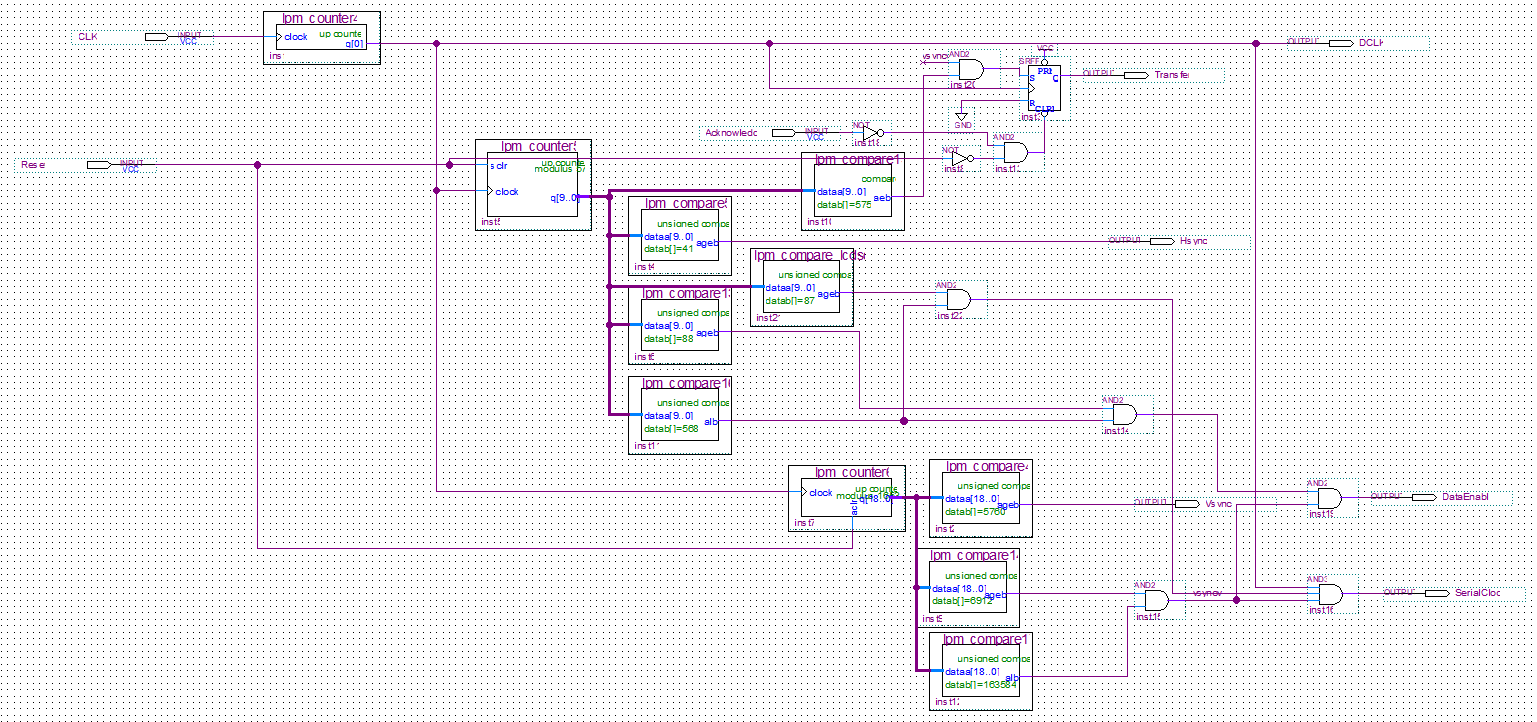
\includegraphics[width=1\textwidth]{{data/LCD_Controller.png}}
	\caption{LCD Controller, with comparators for defining valid regions in the signals.}
	\label{Block:LCD_Controller}    
\end{fullfigure}

\subsubsection{Memory} \index{memory} \label{subsec:Memory}
\marginlabel{Memory Map:} 
%TODO explain? 
\begin{fullfigure} 
	\centering
	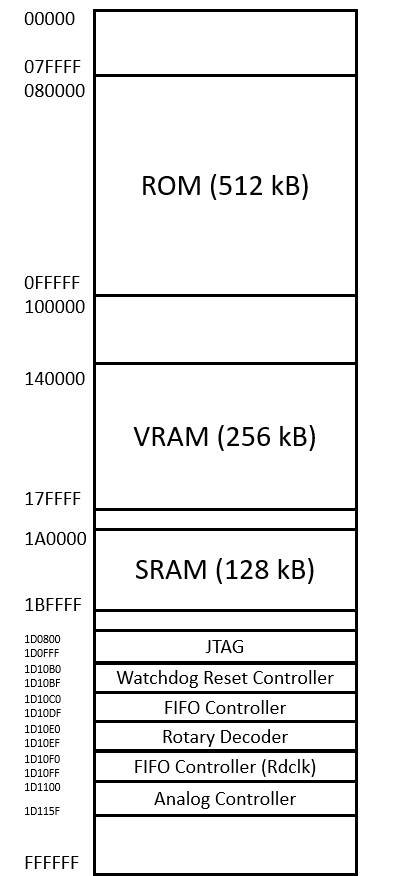
\includegraphics[width=0.4\textwidth]{{data/memorymap.png}}
	\caption{Memory map diagram, used by the CPU(?)} %TODO
	\label{Block:Memorymap}    
\end{fullfigure}

\marginlabel{ROM:} \index{ROM}
1 512 K x 8 bit EEROM (U2, Am29F040) was used. %(to store things?).
8 data bits are connected in parallel through the buffers to the CPU, along with 19 address bits, an active-low chip enable (CE), and output enable (OE) signal. The write enable (WE) signal was pulled up, as the ROM was written to with a dedicated ROM programmer.

The ROM timing diagram for the read cycle can be seen at Appendix~\ref{AP:Timing}, Figure~\ref{AP:ROM_Read_Timing}. 3 read wait states were used. %is this the right way to say it?

The executable file from the Nios II IDE was loaded into it using the ROM programmer. %TODO more??

\begin{fullfigure} 
	\centering
	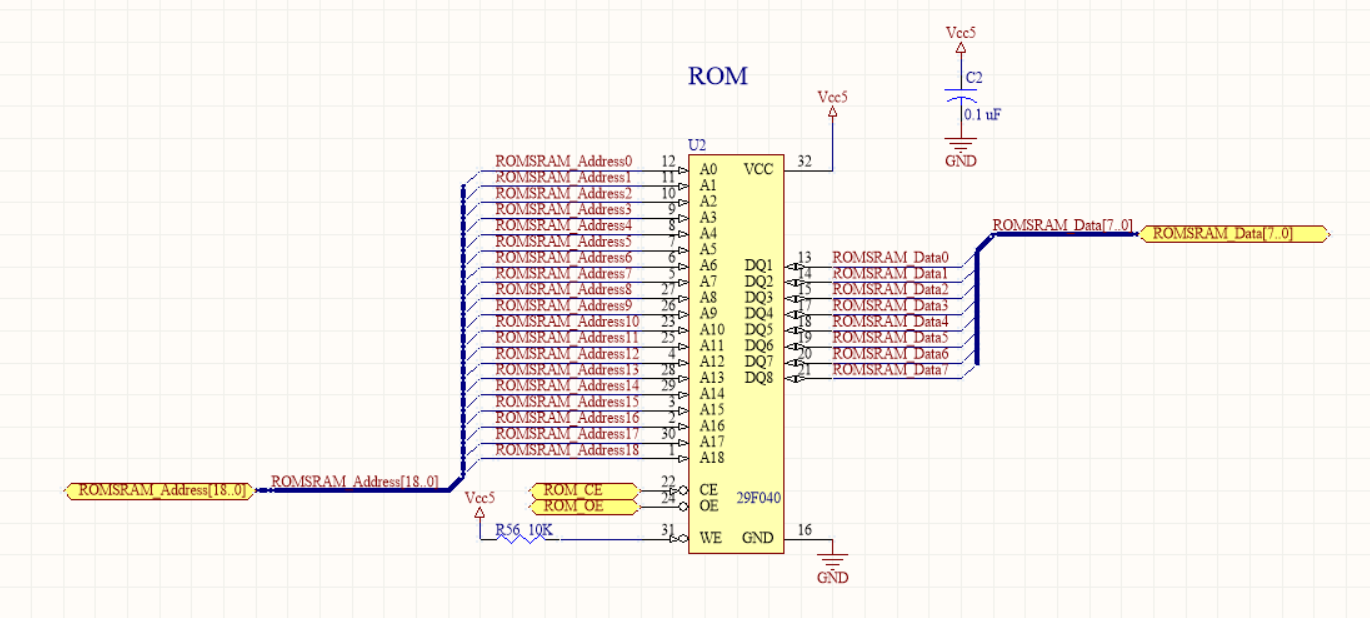
\includegraphics[width=1\textwidth]{{data/ROM.png}}
	\caption{ROM Schematic.}
	\label{Schematic:ROM}    
\end{fullfigure}

%block diagram

\marginlabel{SRAM:} \index{SRAM}
1 128 K x 8 bit CMOS static RAM was used (U1, HM628128B) 

The address line is shared between the ROM and SRAM, with only the 17 least significant bits used for RAM addressing. The 8-bit data bus is also shared between the ROM and SRAM. The active-low output enable (OE), write enable (WE), and chip select (CS1) are also connected between the SRAM and CPU, with the second active high chip select (CS2) pulled high as required by the read and write cycles. 

The SRAM timing diagrams can be seen at Appendix~\ref{AP:Timing},
Figures~\ref{AP:RAM_Read_Timing} and \ref{AP:RAM_Write_Timing}. 2 read wait states and 1 write wait state was used. 

\begin{fullfigure} 
	\centering
	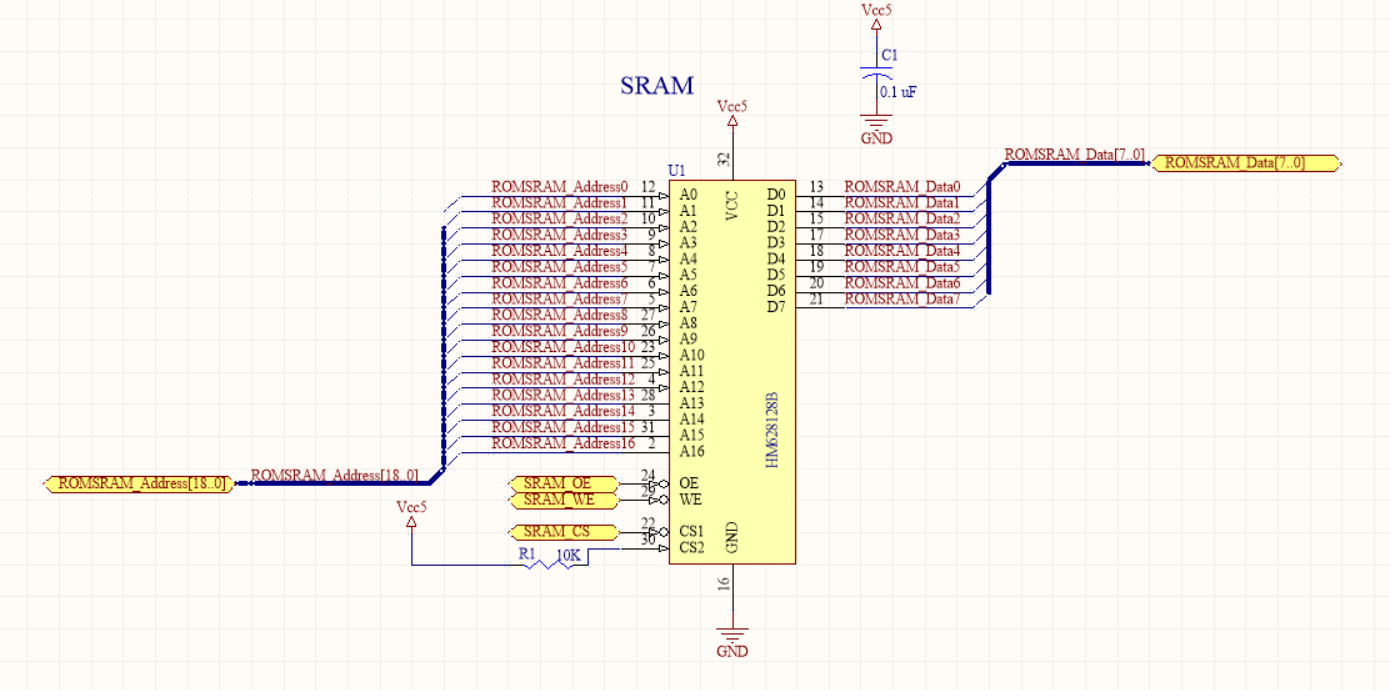
\includegraphics[width=1\textwidth]{{data/SRAM.png}}
	\caption{SRAM Schematic.}
	\label{Schematic:SRAM}    
\end{fullfigure}

\marginlabel{Serial EEPROM:} \index{Serial EEPROM}
A serial configuration device (U4, EPCS16), a 2 MB flash memory device, was used to store FPGA configuration data \footnote{Was unable to successfully use serial device for unknown reasons, possibly due to incorrect FPGA configurations.}.

\begin{fullfigure} 
	\centering
	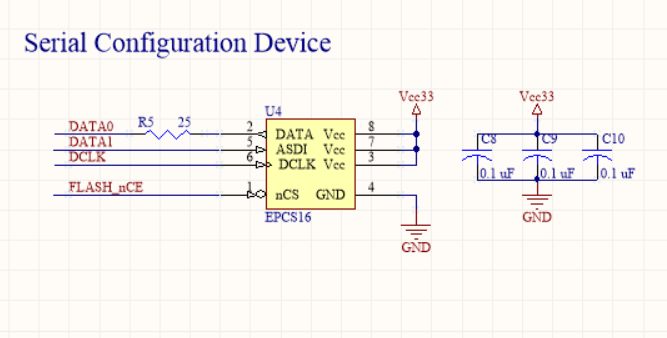
\includegraphics[width=0.75\textwidth]{{data/EEPROM.png}}
	\caption{EEPROM Schematic.}
	\label{Schematic:EEPROM}    
\end{fullfigure}


\subsubsection{FPGA} \index{FPGA}%HERE? idk. talk about controllers 
An Altera Cyclone III FPGA was used (U9, EP3C25Q240). The three required voltage levels were generated with regulators, and each power pin was locally bypassed. 

%level shifters / buffers 
Buffers, or level shifters, were used to connect the buses and control signals from the peripheral chips to the FPGA to go between the low FPGA voltage and mainly 5V environment (U5, U6, U7, U8, U10, U12, 74LVT16245). A separate buffer was used to interface with the ADC (U17, TLC5510A), which had a larger input voltage range requirement (U18, SN74HCT240).

% pinout 
The pins were connected on the PCB as listed in Figure~\ref{}. 
%pinout doc

The final product included several changes. Pin 162, an output for device configuration, was left floating, and the reset input was changed to Pin 187. One buffer was also left unusable, resulting in rewiring to extra I/O pins. 
%pinout excel

\subsubsection{JTAG, Reset, and Clock} \index{Clock} \index{JTAG} \index{Reset} 
% separate? 


pin 162 used during FPGA startup, can't use for reset 

\marginlabel{JTAG:} \index{Reset}

\marginlabel{Reset:} \index{Reset}
A reset circuit is used, which includes a microprocessor supervisory device (U3, MAX705). %more chip details
The watchdog input (WDI) is implemented in the main loop, and a voltage divider is used for a power-fail warning at 4 V from the 5 V supply. 

\marginlabel{Clock:} \index{Reset}

\begin{fullfigure} 
	\centering
	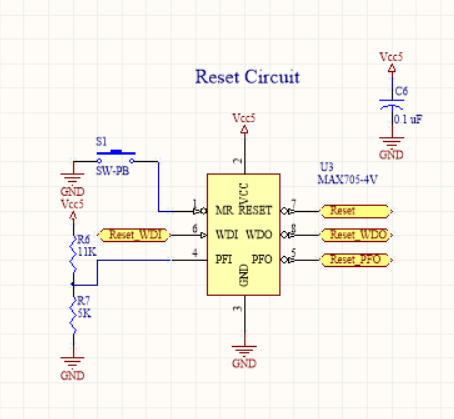
\includegraphics[width=0.6\textwidth]{{data/ResetCircuit.png}}
	\caption{Reset Circuit Schematic.}
	\label{Schematic:Reset}    
\end{fullfigure}

The active-low watchdog output, power-fail output, and reset output, and manual reset output are combined for an overall reset signal that is sent to the CPU and various controllers. 

%schematic pic, fpga pic 

\subsubsection{Fixes}
wrong adc footprint, buffer soldering error, backwards LCD connector

%%%%%%%%%%%%%%%%%%%%%%%%%%%%%%%%%%%%%%%%%%%%%%%%%%%%%%%%%%%%%
\subsection{Software} \index{Software} \label{subsec:software}
\subsubsection{Software System Overview} 
\subsubsection{}

\appendix \index{Appendix}
\section{Code}

\begin{fullpage}\label{AP:scopetrig.vhd} %TODO this will take forever, change
\lstinputlisting[style=VHDLMeUp]{data/scoptrig.vhd} 
\end{fullpage}

\section{Timing Diagrams} \label{AP:Timing} \index{Timing}
\subsection{ADC} %TODO format
	\begin{fullfigure} 
		\centering
		\includegraphics[width=1\textwidth]{{data/timing/ADC.png}}
		\caption{ADC Timing Diagram}
		\label{AP:ADC_Timing}    
	\end{fullfigure}

\subsection{LCD}
\begin{fullfigure} 
	\centering
	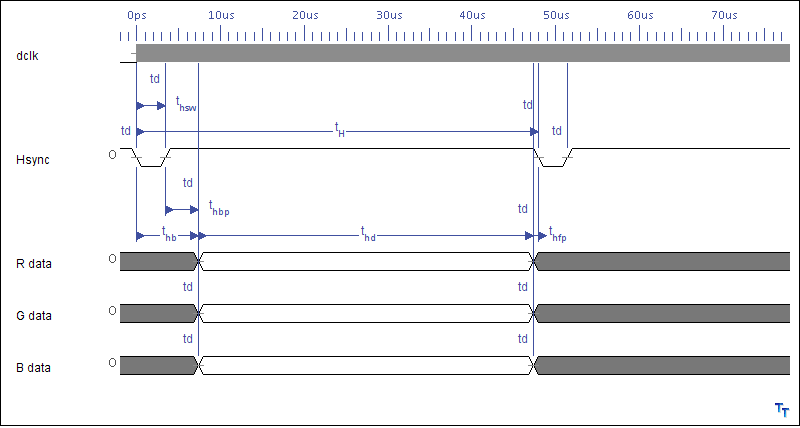
\includegraphics[width=1\textwidth]{{data/timing/LCD_Horizontal.png}}
	\caption{LCD Horizontal Timing Diagram}
	\label{AP:LCD_Horizontal_Timing}    
\end{fullfigure}

\begin{fullfigure} 
	\centering
	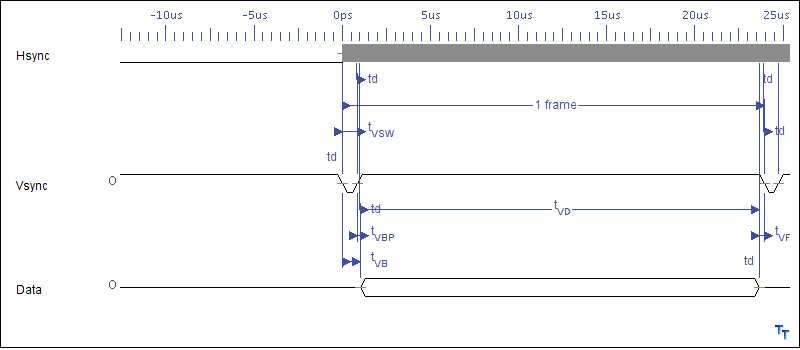
\includegraphics[width=1\textwidth]{{data/timing/LCD_Vertical.png}}
	\caption{LCD Vertical Timing Diagram}
	\label{AP:LCD_Vertical_Timing}    
\end{fullfigure}

\subsection{ROM and RAM}
\begin{fullfigure} 
	\centering
	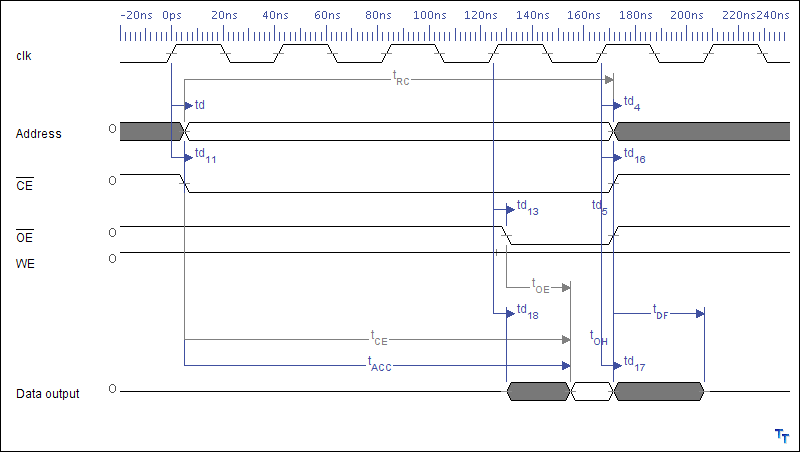
\includegraphics[width=1\textwidth]{{data/timing/ROM_Read.png}}
	\caption{ROM Read Cycle Diagram}
	\label{AP:ROM_Read_Timing}    
\end{fullfigure}

\begin{fullfigure} 
	\centering
	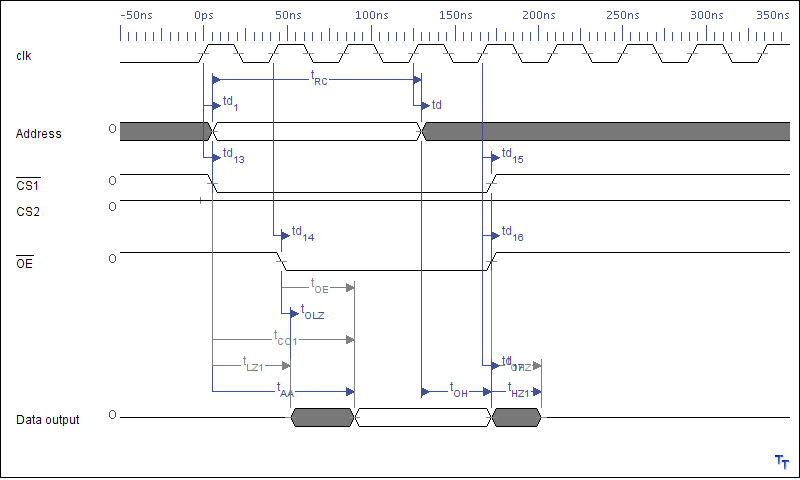
\includegraphics[width=1\textwidth]{{data/timing/SRAM_Read.png}}
	\caption{RAM Read Cycle Diagram}
	\label{AP:RAM_Read_Timing}    
\end{fullfigure}

\begin{fullfigure} 
	\centering
	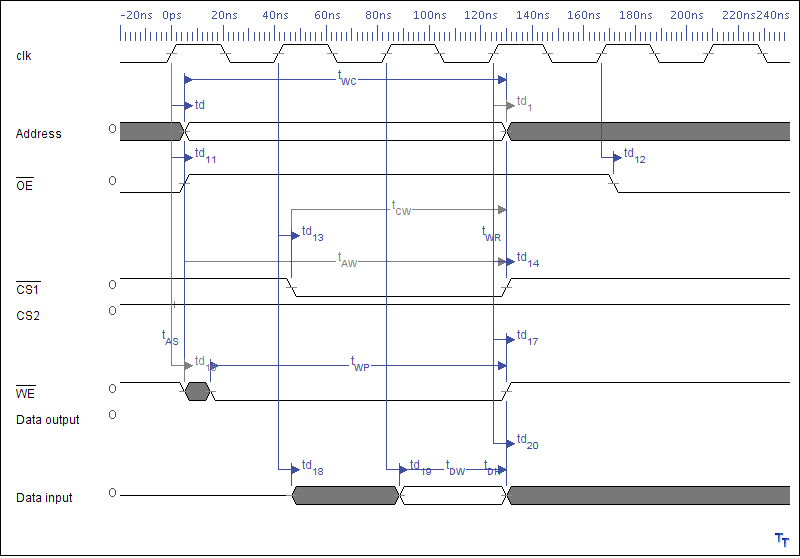
\includegraphics[width=1\textwidth]{{data/timing/SRAM_Write.png}}
	\caption{RAM Write Cycle Diagram}
	\label{AP:RAM_Write_Timing}    
\end{fullfigure}

\subsection{VRAM}
\begin{fullfigure} 
	\centering
	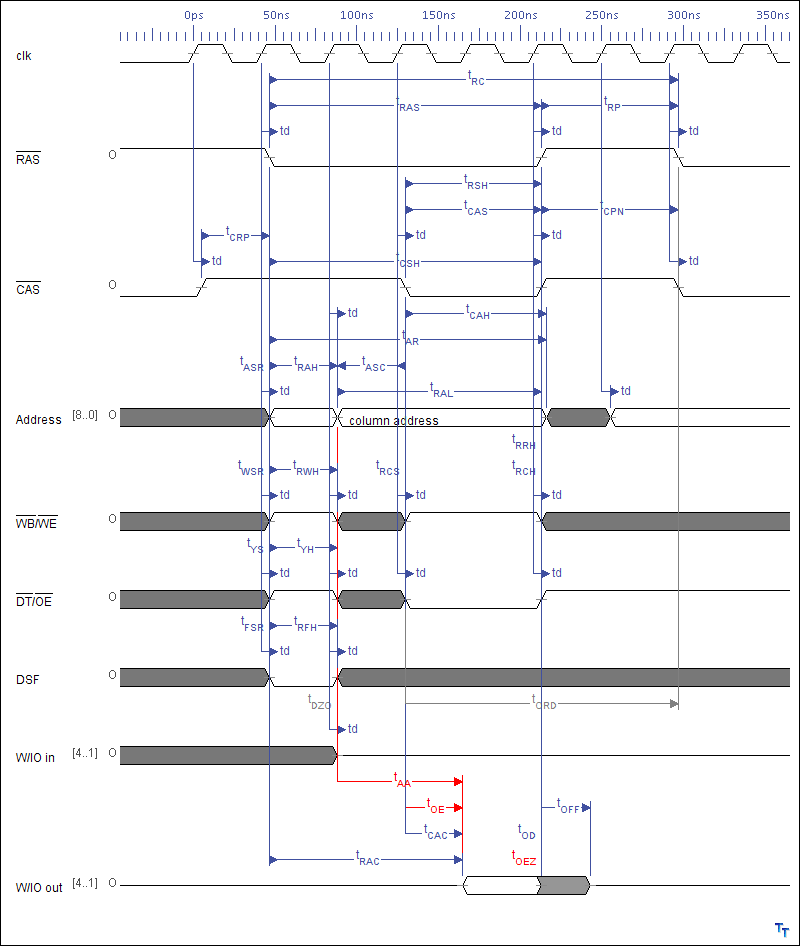
\includegraphics[width=1\textwidth]{{data/timing/VRAM_Read_MT.png}}
	\caption{VRAM Read Cycle Diagram}
	\label{AP:VRAM_Read_Timing}    
\end{fullfigure}

\begin{fullfigure} 
	\centering
	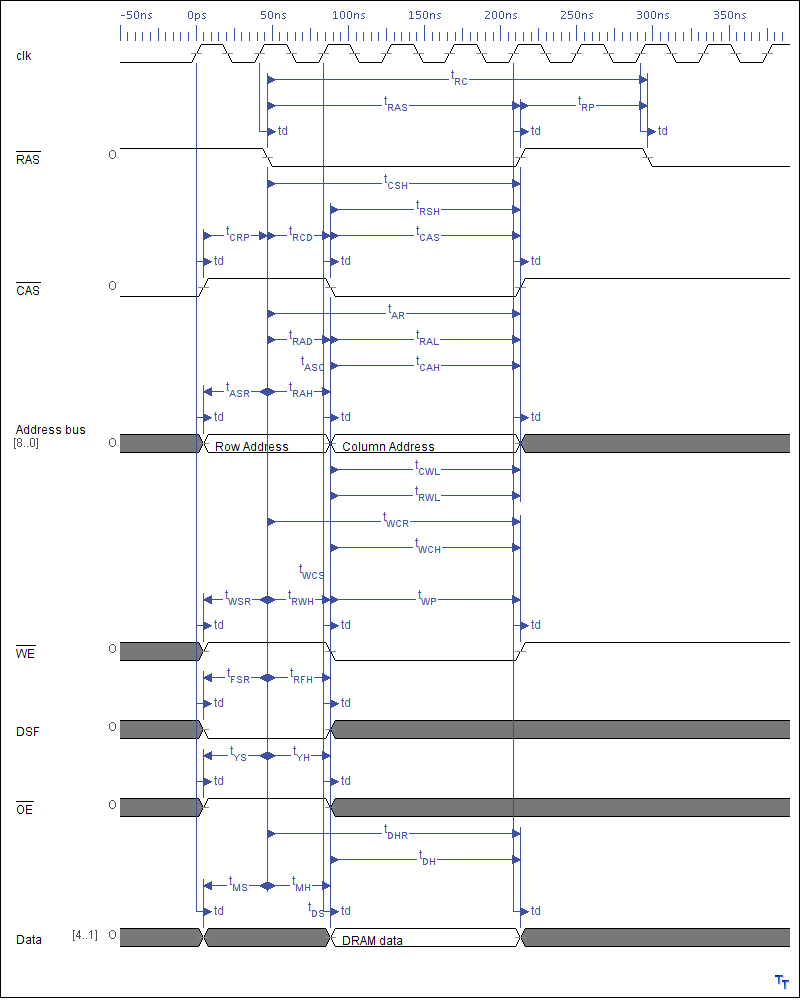
\includegraphics[width=1\textwidth]{{data/timing/VRAM_Write_MT.png}}
	\caption{VRAM Write Cycle Diagram}
	\label{AP:VRAM_Write_Timing}    
\end{fullfigure}

\begin{fullfigure} 
	\centering
	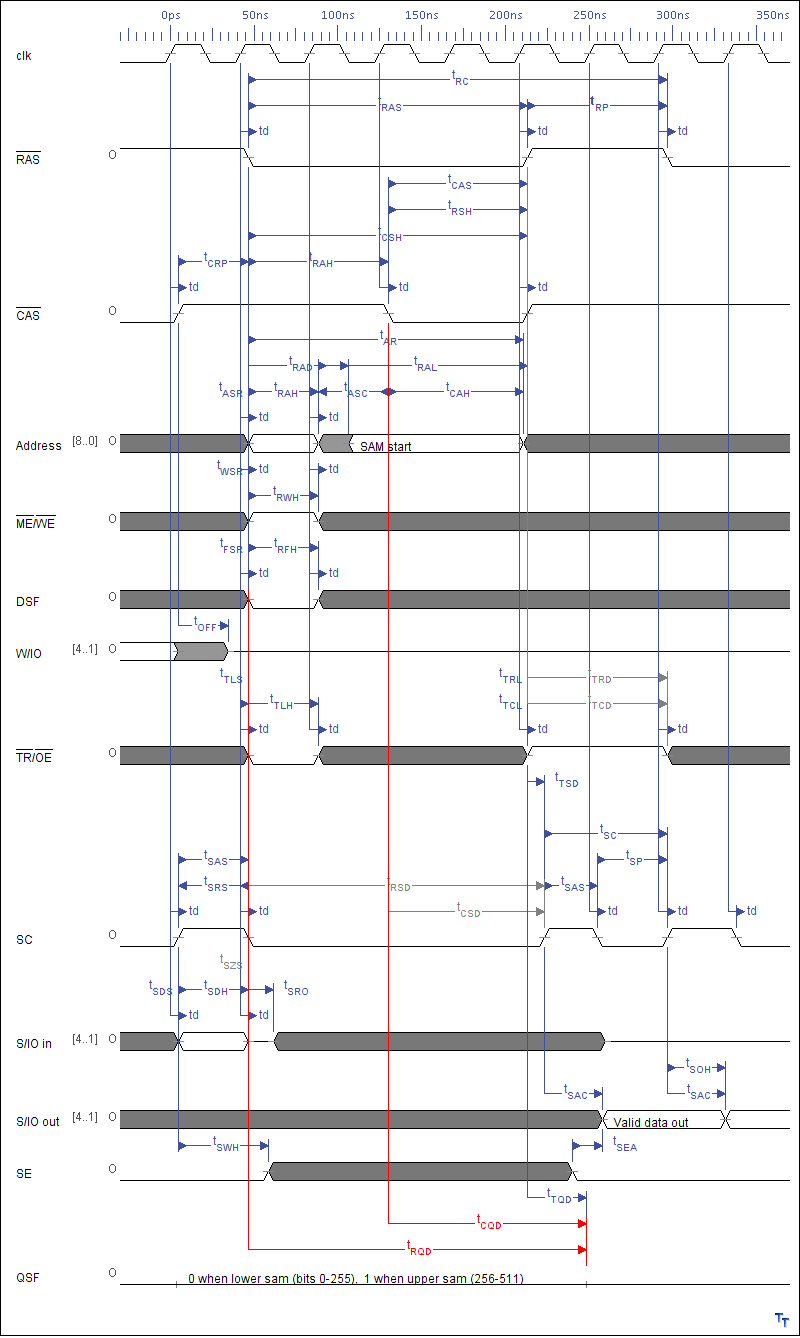
\includegraphics[width=0.75\textwidth]{{data/timing/VRAM_Read_Transfer_MT.png}}
	\caption{VRAM Row Transfer Cycle Diagram}
	\label{AP:VRAM_Transfer_Timing}    
\end{fullfigure}

\begin{fullfigure} 
	\centering
	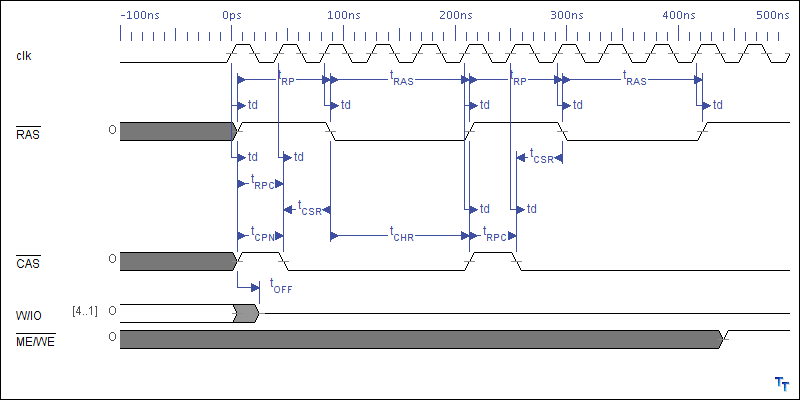
\includegraphics[width=1\textwidth]{{data/timing/VRAM_refresh_MT.png}}
	\caption{VRAM Refresh Cycle Diagram (CAS before RAS)}
	\label{AP:VRAM_Refresh_Timing}    
\end{fullfigure}

\begin{fullfigure} 
	\centering
	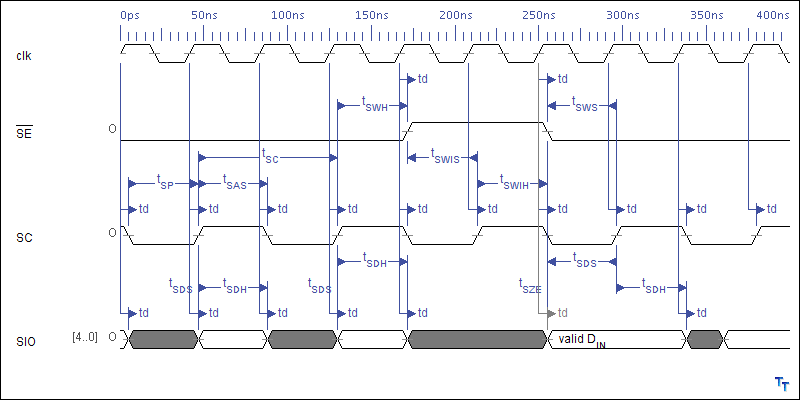
\includegraphics[width=1\textwidth]{{data/timing/VRAM_Serial_Write_MT.png}}
	\caption{VRAM Serial Write Cycle Diagram}
	\label{AP:VRAM_Serial_Write_Timing}    
\end{fullfigure}


\begin{comment}
\begin{figure} [H]
\centering
\includegraphics[width=0.75\textwidth]{{data/ADC.png}}
\caption{}
\label{ADC_Timing}    
\end{figure}
\end{comment}
%\appendix 
% entire schematic 
% list of changes to pcb and glen's code 
\printindex 
\end{document}


\begin{comment}

\begin{description}

\item[Line spacing]\index{line spacing}

\end{description}

\attention

\footnote{text}

\index{}\marginlabel{}

\texttt{}

\begin{figure} [H]
\centering
\includegraphics[width=0.75\textwidth]{{data/}}
\caption{block diagram}
\label{LCDBlockDiagram}    
\end{figure}


\usepackage{pdfpages}

\includepdf[pages={1}]{myfile.pdf} 
pages={-} 
for all 
\end{comment}